\documentclass{beamer}

\mode<presentation> {
\usetheme{Madrid}
\setbeamertemplate{navigation symbols}{}
}

\usepackage{graphicx}
\usepackage{booktabs}
\usepackage[utf8]{inputenc}
\usepackage{subfigure}
\usepackage{amsmath}
\usepackage{array}
\usepackage[]{algorithm2e}
\usepackage{caption}
\usepackage{subcaption}

\setbeamertemplate{caption}[numbered]

\newcommand{\norm}[1]{\left\lVert#1\right\rVert}

\title[Reinforcement Learning]{Reinforcement Learning}
\author[Rasmus Holm]{Rasmus Holm}
\institute[LiU]{
Linköping University \\
}
\date{\today}

\begin{document}
    %----------------------------------------------------------------------------------------
    %	INTRODUCTION SLIDES
    %----------------------------------------------------------------------------------------

    \begin{frame}
        \titlepage
    \end{frame}

    \begin{frame}
        \frametitle{Overview}
        \tableofcontents
    \end{frame}
    %----------------------------------------------------------------------------------------
    %	PRESENTATION SLIDES
    %----------------------------------------------------------------------------------------

    \section{Introduction}

    \begin{frame}
        \frametitle{Introduction}
    \end{frame}

    \begin{frame}
        \frametitle{Use Cases}
    \end{frame}

    \section{Motivation}
    \begin{frame}
        \frametitle{Motivation}
    \end{frame}

    \begin{frame}
        \frametitle{Datasets}
        \begin{columns}
            \column{0.4\linewidth}
            \begin{itemize}
                \item Choi
                \item Cenlab
                \item New York Times
                \item State of the Union
            \end{itemize}
            \column{0.6\linewidth}
            \begin{table}[t]
                \centering
                \resizebox{\columnwidth}{!}{%
                \begin{tabular}{lrrrr}
                    \toprule
                    Corpus & $D$ & $P$ & $N$ & $V$ \\
                    \midrule
                    Choi & 300 & 3000 & 251528 & 6537 \\
                    Cenlab & 377 & 599817 & 13392815 & 303765 \\
                    NYT2007 & 36639 & 471001 & 11475158 & 240238 \\
                    SOTU & 212 & 19232 & 693698 & 26074 \\
                    \bottomrule
                \end{tabular}
                }
                \label{tab:corpora}
            \end{table}
        \end{columns}
    \end{frame}

    \section{Topic Models}

    \begin{frame}
        \frametitle{Latent Dirichlet Allocation}
        LDA Generative Process (Blei et al., 2003)
        \newline

        \begin{algorithm}[H]
            \KwData{Number of topics $\mathbf{K}$, Vocabulary size $\mathbf{V}$, Document size $\mathbf{N}$}

            Choose $\mathbf{\theta} \sim Dir(\mathbf{\alpha})$, $\theta \in [0, 1]^{1 \times K}$ \\
            Choose $\mathbf{\phi_{z}} \sim Dir(\mathbf{\beta})$, $\phi \in [0, 1]^{K \times V}$ \\
            \For{each position $\mathbf{i} = 1$ to $\mathbf{N}$}{
            Choose a topic $\mathbf{z_i} \sim Multinomial(\theta)$ \\
            Choose a word $\mathbf{w_i} \sim Multinomial(\mathbf{\phi_{z_i}})$
            }
        \end{algorithm}

        \begin{equation*}
            \begin{array}{ccccc}
                \theta | W &=
                \begin{bmatrix}
                    \theta_{11} & \cdots & \theta_{1K} \\
                    \vdots &\ddots & \vdots \\
                    \theta_{D1} & \cdots & \theta_{DK}
                \end{bmatrix} &

                \phi | W &=
                \begin{bmatrix}
                    \phi_{11} & \cdots & \phi_{1V} \\
                    \vdots &\ddots & \vdots \\
                    \phi_{K1} & \cdots & \phi_{KV}
                \end{bmatrix} \\
                & \text{$D \times K$} & & \text{$K \times V$}
            \end{array}
        \end{equation*}
    \end{frame}

    \section{Backup Diagrams}

    \begin{frame}
        \begin{figure}[ht]
            \centering
            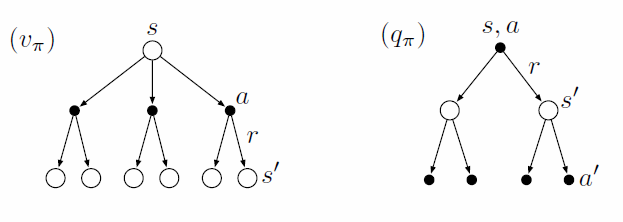
\includegraphics[width=\linewidth]{./images/backup_diagrams.PNG}
            \caption{Backup diagrams for state-value function and action-value function.}
            \label{fig:backup_diagrams}
        \end{figure}
    \end{frame}

    \section{Evaluation}

    \begin{frame}
        \frametitle{Evaluation}
    \end{frame}

    \begin{frame}
        \frametitle{Held-out Marginal Likelihood}
        Left-to-Right evaluation (Wallach et al., 2009)
        \newline

        \begin{algorithm}[H]
            \KwData{Document $\mathbf{d}$, Model $\mathbf{m}$, Number of Particles $\mathbf{R}$}
            \KwResult{Estimated likelihood $\mathbf{l} = p(\mathbf{d} | \mathbf{m})$}
            initialize $\mathbf{l} = 0$ \\
            \For{each position $\mathbf{n}$ in document $\mathbf{d}$}{
            initialize $\mathbf{p_n} = 0$ \\
            \For{each particle $\mathbf{r} = 1$ to $\mathbf{R}$}{
            \For{each position $\mathbf{n^\prime} < \mathbf{n}$}{
            sample topic $\mathbf{z_{n^\prime}} \sim p(\mathbf{z_{n^\prime}} | \mathbf{w_{n^\prime}}, \{ \mathbf{z_{< n}}\}_{\backslash \mathbf{n^\prime}}, \mathbf{m})$
            }

            $\mathbf{p_n} = \mathbf{p_n} + \sum_t p(\mathbf{w_n}, \mathbf{z_n} = t | \mathbf{z_{< n}}, \mathbf{m})$ \\
            sample $\mathbf{z_n} \sim p(\mathbf{z_n} | \mathbf{z_n}, ), \mathbf{z_{< n}}, \mathbf{m})$
            }
            $\mathbf{l} = \mathbf{l} + \log(\frac{\mathbf{p_n}}{\mathbf{R}})$
            }
        \end{algorithm}
    \end{frame}

    \section{Conclusion}

    \begin{frame}
        \frametitle{Conclusion}

    \end{frame}

    \begin{frame}
        \Huge{\centerline{The End}}
    \end{frame}

\end{document}
